\documentclass[11pt]{article}
\usepackage[a4paper,margin=2.6cm]{geometry}
\usepackage[T1]{fontenc}
\usepackage[utf8]{inputenc}
\usepackage{times}
\usepackage{microtype}
\usepackage{booktabs}
\usepackage{graphicx}
\usepackage{amsmath,amssymb}
\usepackage{xcolor}
\usepackage[numbers,sort&compress]{natbib}
\usepackage[hidelinks]{hyperref}
\usepackage{caption}
\usepackage{enumitem}
\captionsetup{font=small,labelfont=bf}
\setlist{nosep}
\setlength{\emergencystretch}{3em}

\renewcommand{\Box}{\square}
\newcommand{\Dia}{\lozenge}

\title{Constrained Decoding Makes Guesses Look Canonical:\\
\large Formal validity without semantic correctness in small-model Kripke judgements}

\author{Bart{\l}omiej Nawara\\
Independent researcher, Poland\\
\texttt{barteknawara@gmail.com}}

\date{September 2026}

\begin{document}
\maketitle

\begin{abstract}
Decode-time constraints guarantee that a language model's output belongs to a fixed set of well-formed strings. They say nothing about whether the string is true. We measure the gap on a small, fully synthetic task: given a four-world Kripke model and a target world, emit the canonical judgement ``$w_i \models \varphi$ iff TRUE/FALSE'' for a modal formula $\varphi$. Two instruction-tuned models (Qwen2.5-0.5B and 1.5B) are run under five arms: unconstrained, format-prompted, format-prompted with a stricter template, and the two prompted arms with a byte-trie constraint that admits only canonical judgements. The constraint does what it promises. Membership violations fall from 42--114 per 160 fixtures to zero, and strict exact-match rises from 8--26 to 51--52 of 80 in-language fixtures (paired exact McNemar $p<10^{-7}$). That headline is misleading in three ways, all visible once outputs are re-parsed leniently and the constraint set is inspected. First, the constraint set was built from the gold judgements and admits only one truth value for 25 of the 80 fixtures; on those the constraint cannot be wrong. On the 55 fixtures where both truth values are admissible, constrained accuracy is 26/55 and 27/55, indistinguishable from chance (binomial $p=0.79$, $1.00$). Second, each model emits an almost constant truth value regardless of arm: the 0.5B model answers TRUE on 80 of 80 prompted and 55 of 55 free constrained fixtures, the 1.5B model answers FALSE on 73 of 80 and 51 of 55. Per-formula accuracy tracks the gold base rate of that constant, not the formula. Third, under a lenient parser the unconstrained 1.5B model already gets the world and formula right on 79 of 80 fixtures and reaches 42/80 semantic accuracy; strict scoring had reduced it to 25 because of underscores and spaces. Neither model ever abstains on the 80 out-of-language fixtures; the constraint turns every one into a fluent, in-language, spurious judgement. Constrained decoding here converts a coin flip into a syntactically perfect coin flip, and membership-only evaluation cannot tell the difference. We release fixtures, code, cached outputs and the re-analysis, and add a leak-free constraint construction to the pipeline.
\end{abstract}

\section{Introduction}

Structured generation is now a standard component of LLM pipelines. A grammar, a JSON schema or a finite set of admissible strings is compiled into a mask on the next-token distribution, and the model is guaranteed to produce a well-formed output \citep{willard2023outlines,geng2023grammar}. The guarantee is syntactic. Whether it improves, leaves alone, or degrades the semantic content of the output is an empirical question that has mostly been studied on tasks where the answer is a free-text span or a number \citep{tam2024speak}. We study it on a task where the well-formed outputs are few, enumerable, and each one is either true or false under a precise semantics: truth of modal formulas at worlds of a Kripke model \citep{kripke1963,blackburn2001modal}.

The task is deliberately tiny. Four worlds, one accessibility relation, a valuation for two atoms, a target world, a target formula built from $\Box$, $\Dia$, $\neg$ and $\wedge$. The answer is one of two strings. A model that understood the semantics would get it right; a model that did not would be at 50\%. Between those two poles there is a lot of room for a decoding method to make a guess look like an answer, and for a scorer to reward it.

Our pipeline scores outputs in migration classes: exact, canonical-but-wrong, non-canonical, and (for fixtures whose formula uses an atom outside the language) spurious judgement versus correct abstention. Under that scorer, constrained decoding wins decisively, and the paired McNemar test agrees at $p<10^{-7}$. This paper is about why that result should not be believed as stated, and what one has to look at to see through it. Three things, in order: the constraint set itself, the truth-value distribution of the outputs, and the parser.

We make the following contributions.
\begin{enumerate}
  \item A 160-fixture Kripke judgement benchmark with deterministic construction, a canonical output language, and a byte-trie constraint that admits exactly that language, running on the \texttt{transformers} \texttt{LogitsProcessor} interface (Section~\ref{sec:setup}).
  \item Five-arm results for two small instruction-tuned models, with the pipeline's own membership-based scoring (Section~\ref{sec:primary}).
  \item A re-analysis showing that (a) the constraint set leaks the answer on 31\% of fixtures, (b) on the remaining fixtures constrained accuracy is at chance, (c) both models emit a near-constant truth value, and (d) lenient parsing reveals the unconstrained models already produce the right structure (Sections~\ref{sec:leak}--\ref{sec:lenient}).
  \item A leak-free constraint construction, added to the released pipeline, and a recommended evaluation protocol for constrained decoding on tasks with a semantic ground truth (Section~\ref{sec:discussion}).
\end{enumerate}

\section{Related work}

Guided or constrained decoding restricts the next-token distribution to the continuations licensed by a grammar or automaton \citep{willard2023outlines,geng2023grammar}; the finite-set variant we use is the degenerate case where the grammar is a trie over a fixed list of strings. \citet{tam2024speak} report that format restrictions can lower reasoning accuracy on arithmetic and commonsense benchmarks; our setting differs in that the admissible set is so small that any effect of the constraint on reasoning is dwarfed by the model's prior over the two truth values. \citet{holliday2024modal} evaluate large models on conditional and modal inference in natural language and find systematic failures on modal patterns; we evaluate much smaller models on the explicit possible-worlds semantics rather than on natural-language modals. The models are from the Qwen2.5 family \citep{qwen2.5}. Paired comparisons use the exact McNemar test \citep{mcnemar1947} and bootstrap intervals \citep{efron1993bootstrap}.

\section{Task, data and arms}
\label{sec:setup}

\paragraph{Fixtures.} The language has atoms $p$ and $q$, connectives $\neg$ and $\wedge$, and modalities $\Box$ and $\Dia$, written in the prompt as \texttt{NOT}, \texttt{AND}, \texttt{BOX}, \texttt{DIA}. There are five accessibility relations over worlds $w_0..w_3$, four valuations, and four in-language formulas: $\Box p$, $\Dia q$, $\neg\Box\neg p$, and $\Box p \wedge \Dia q$. The Cartesian product gives 80 in-language fixtures; the target world is $w_{(i+j+k) \bmod 4}$ for frame $i$, valuation $j$, formula $k$. Truth is computed by the standard clauses ($\Box\varphi$ true at $w$ iff $\varphi$ true at every $R$-successor of $w$). A second block of 80 fixtures uses the same frames and valuations with formulas containing an atom $r$ that has no valuation ($\Box r$, $\Dia r$, $\neg r$, $p \wedge r$); the prompt says so, and the correct output is the empty string. Gold truth values over the 80 in-language fixtures are 44 FALSE and 36 TRUE, unevenly across formulas: $\neg\Box\neg p$ is TRUE in 18 of 20 cases, $\Box p \wedge \Dia q$ is FALSE in 18 of 20.

\paragraph{Canonical output.} \texttt{w\_i |= FORMULA iff TRUE.} or the same with \texttt{FALSE}, with the formula text exactly as given. The pipeline's admissible set $\mathcal{A}$ is the set of gold judgements of the 80 in-language fixtures. Because several fixtures share a (world, formula) pair, $|\mathcal{A}| = 27$. The consequences of building $\mathcal{A}$ this way are the subject of Section~\ref{sec:leak}.

\paragraph{Models and arms.} \texttt{Qwen2.5-0.5B-Instruct} and \texttt{Qwen2.5-1.5B-Instruct}, bfloat16, greedy decoding, at most 64 new tokens, via \texttt{transformers} 4.56 on CUDA. Five arms per model: \emph{naive} (model description, task, the fixture text, and the instruction to output one judgement); \emph{prompted} (adds one line giving the exact format); \emph{prompt\_tuned} (adds a five-line template and an explicit instruction to output empty on out-of-language atoms); \emph{constrained} and \emph{constrained\_tuned} (the two prompted arms plus a logits processor that masks every token not consistent with some string in $\mathcal{A}$, resynchronising to the trie root if the prefix leaves the trie, and admitting EOS only once a full canonical string has been emitted, or immediately for out-of-language fixtures). Prompts are in Appendix~\ref{app:prompt}. Every arm ran on all 160 fixtures; 1,600 outputs in total.

\paragraph{Scoring.} A strict regular expression extracts the first canonical judgement (\texttt{w\textbackslash d+}, \texttt{|=}, a formula with no spaces, \texttt{iff}, \texttt{TRUE|FALSE}). Outputs are classed as \emph{exact} (parsed string equals gold), \emph{valid\_wrong\_judgement} (parsed string in $\mathcal{A}$ but not gold), \emph{invented\_schema} (no parse, or parse not in $\mathcal{A}$), \emph{valid\_spurious\_judgement} (in $\mathcal{A}$ on an out-of-language fixture), \emph{abstention} (empty on an in-language fixture) and \emph{correct\_abstain} (empty on an out-of-language fixture). The pipeline reports class counts and an exact McNemar test on strict exact-match between the prompted and constrained arms.

\section{Results as the pipeline reports them}
\label{sec:primary}

\begin{table}[t]
\centering
\caption{Class counts per model and arm as produced by the pipeline's strict scorer (160 fixtures: 80 in-language, 80 out-of-language). Abstention and correct abstention are zero in every cell and omitted. Membership violations count parsed outputs not in $\mathcal{A}$.}
\label{tab:classes}
\footnotesize
\setlength{\tabcolsep}{4pt}
\begin{tabular}{llrrrrrr}
\toprule
Model & Arm & exact & valid, wrong & not canonical & spurious & membership viol. & format viol. \\
\midrule
0.5B & naive & 0 & 0 & 160 & 0 & 0 & 160 \\
0.5B & prompted & 26 & 19 & 115 & 0 & 114 & 1 \\
0.5B & prompt\_tuned & 19 & 17 & 124 & 0 & 107 & 17 \\
0.5B & constrained & 51 & 29 & 0 & 80 & 0 & 0 \\
0.5B & constrained\_tuned & 51 & 29 & 0 & 80 & 0 & 0 \\
\midrule
1.5B & naive & 25 & 24 & 111 & 0 & 56 & 55 \\
1.5B & prompted & 8 & 6 & 146 & 0 & 42 & 104 \\
1.5B & prompt\_tuned & 0 & 0 & 160 & 0 & 0 & 160 \\
1.5B & constrained & 52 & 28 & 0 & 80 & 0 & 0 \\
1.5B & constrained\_tuned & 52 & 28 & 0 & 80 & 0 & 0 \\
\bottomrule
\end{tabular}
\end{table}

Table~\ref{tab:classes} and Figure~\ref{fig:classes} give the picture the pipeline draws. The constraint removes every membership and format violation. Strict exact-match on the 80 in-language fixtures rises from 26 to 51 (0.5B) and from 8 to 52 (1.5B). The paired exact McNemar test between prompted and constrained reports 0 fixtures where only the prompted arm is right against 25 (0.5B) and 44 (1.5B) where only the constrained arm is right, $p = 6\times10^{-8}$ and $1\times10^{-13}$. The tuned prompt does not help: on the 1.5B model it drives strict exact-match to zero, because the model starts writing \texttt{w\_0} with an underscore. Constrained and constrained\_tuned produce different strings on 49 and 69 of 160 fixtures, almost all on the out-of-language block, and identical strict exact-match sets on the 0.5B model (two fixtures differ on the 1.5B).

\begin{figure}[t]
\centering
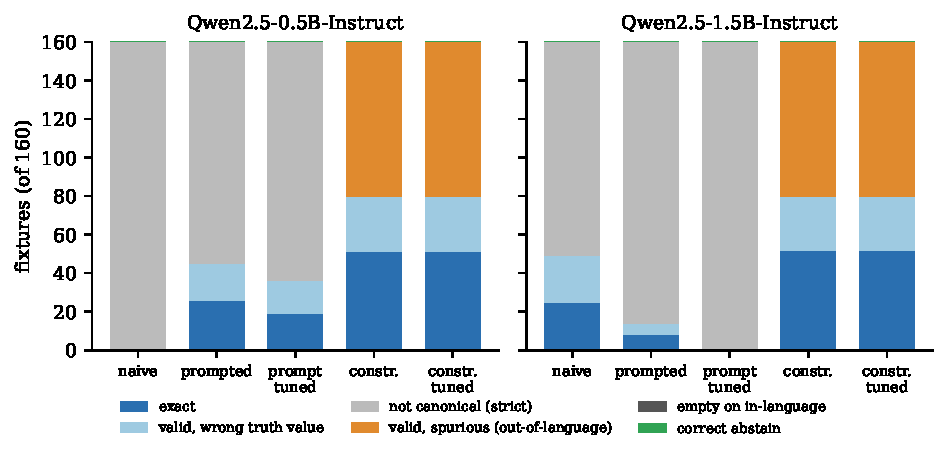
\includegraphics[width=\linewidth]{figs/class_counts.pdf}
\caption{Strict migration classes per arm. Constraint arms have no non-canonical outputs and no abstentions; every out-of-language fixture becomes a spurious in-language judgement.}
\label{fig:classes}
\end{figure}

If we stopped here, the conclusion would be that a decode-time constraint roughly doubles the accuracy of small models on modal judgement. Three checks show that this is not what happened.

\section{Check 1: the constraint set leaks the answer}
\label{sec:leak}

$\mathcal{A}$ contains the 27 distinct gold strings. For a fixture with target world $w$ and formula $\varphi$, the constraint admits \texttt{w |= $\varphi$ iff TRUE.} only if some fixture in the set has that gold judgement, and likewise for FALSE. For 5 of the 16 (world, formula) pairs, only one truth value ever occurs in gold: $(w_2, \Box p)$ is always FALSE, $(w_1, \neg\Box\neg p)$ and $(w_2, \neg\Box\neg p)$ always TRUE, $(w_1, \Box p\wedge\Dia q)$ and $(w_2, \Box p\wedge\Dia q)$ always FALSE. Those pairs cover 25 of the 80 in-language fixtures. On them the trie admits exactly one complete string with the target world and formula, and since both models always reproduce the target world and formula under the constraint (80 of 80, Section~\ref{sec:bias}), the constrained arm cannot be wrong. We call these fixtures \emph{forced} and the other 55 \emph{free}.

\begin{table}[t]
\centering
\caption{In-language accuracy split by whether the trie admits both truth values. Constrained arms use strict exact-match; unconstrained arms use the lenient parser of Section~\ref{sec:lenient}. Two-sided binomial $p$ against 0.5 on the free set.}
\label{tab:forcedfree}
\small
\begin{tabular}{llrrrr}
\toprule
Model & Arm & forced ($n{=}25$) & free ($n{=}55$) & free acc. & $p$ vs chance \\
\midrule
0.5B & naive (lenient) & 0 & 0 & 0.000 & $<0.001$ \\
0.5B & prompted (lenient) & 10 & 18 & 0.327 & 0.014 \\
0.5B & prompt\_tuned (lenient) & 7 & 13 & 0.236 & $<0.001$ \\
0.5B & constrained & 25 & 26 & 0.473 & 0.79 \\
\midrule
1.5B & naive (lenient) & 12 & 30 & 0.545 & 0.59 \\
1.5B & prompted (lenient) & 13 & 27 & 0.491 & 1.00 \\
1.5B & prompt\_tuned (lenient) & 7 & 18 & 0.327 & 0.014 \\
1.5B & constrained & 25 & 27 & 0.491 & 1.00 \\
\bottomrule
\end{tabular}
\end{table}

Table~\ref{tab:forcedfree} and Figure~\ref{fig:forcedfree} split the in-language accuracy accordingly. Constrained arms score 25/25 on the forced fixtures, as they must, and 26/55 and 27/55 on the free ones. Neither free-set accuracy differs from a fair coin (binomial $p = 0.79$ and $1.00$). Of the 51--52 strict exact matches the pipeline credits to constrained decoding, 25 are supplied by the constraint set, and the rest are what a coin would supply. The pipeline's McNemar result is arithmetically correct and inferentially empty: it compares a coin that always lands in the admissible set against outputs that are often thrown out for an underscore.

\begin{figure}[t]
\centering
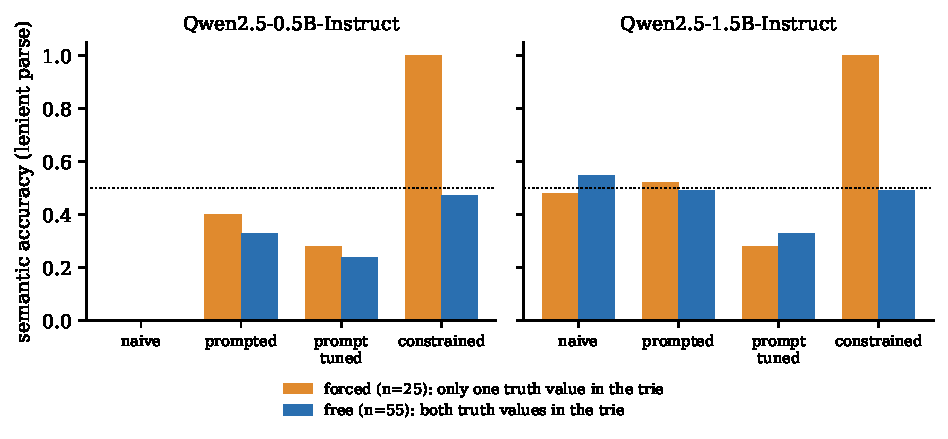
\includegraphics[width=0.92\linewidth]{figs/forced_vs_free.pdf}
\caption{Semantic accuracy on forced fixtures (only one truth value admissible) and free fixtures (both admissible). Dotted line: chance. Constrained decoding is perfect where it cannot be wrong and at chance where it can.}
\label{fig:forcedfree}
\end{figure}

The leak is a construction error, not a property of constrained decoding. The admissible set should have been the full product of worlds, formulas and truth values (32 strings), or, equivalently, the gold strings together with their truth-value complements. We have added that construction to the pipeline as \texttt{--allowed-set product} (Section~\ref{sec:repro}); the experiments in this paper were not re-run with it, and the forced/free split above is the correction we can make from the cached outputs.

\section{Check 2: the truth value is a constant}
\label{sec:bias}

The free-set numbers are not merely at chance; they are at chance for a specific reason. Figure~\ref{fig:bias} shows the distribution of the emitted truth value on the 55 free fixtures. The 0.5B model answers TRUE on 55 of 55 under the constraint and on 80 of 80 in-language fixtures under the prompted arm. The 1.5B model answers FALSE on 51 of 55 under the constraint, and on 73 of 80 prompted and 75 of 80 naive. The constant is a property of the model, not of the arm: the constraint does not change which truth value the model prefers, it only guarantees that the preference is spelled correctly.

\begin{figure}[t]
\centering
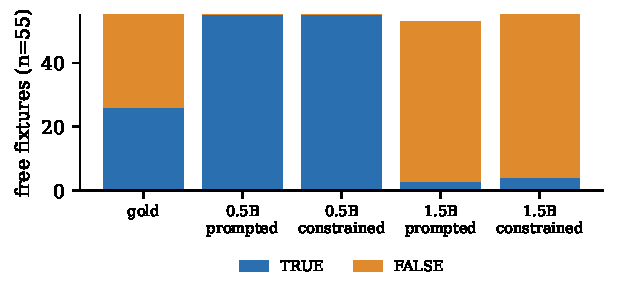
\includegraphics[width=0.62\linewidth]{figs/truth_value_bias.pdf}
\caption{Emitted truth value on the 55 free fixtures. Gold is 26 TRUE / 29 FALSE. The 0.5B model says TRUE; the 1.5B model says FALSE; the arm barely matters.}
\label{fig:bias}
\end{figure}

This explains the per-formula pattern, which would otherwise look like partial understanding. On the 0.5B model, constrained accuracy is 18/20 on $\neg\Box\neg p$ and 8/20 on $\Box p$; on the 1.5B model it is 16/20 on $\Box p\wedge\Dia q$, 17/20 on $\Box p$ and 7/20 on $\Dia q$. Every one of these numbers is the gold base rate of the model's constant: $\neg\Box\neg p$ is TRUE 18 of 20 times and the 0.5B model says TRUE; $\Box p\wedge\Dia q$ is FALSE 18 of 20 times and the 1.5B model says FALSE. A model that had learned that $\Dia$ statements are usually satisfiable in dense frames would show the same profile. So would one that had learned nothing. The fixture design, with its skewed truth distribution per formula, cannot distinguish them, and neither can accuracy.

\section{Check 3: the parser was doing most of the work}
\label{sec:lenient}

The strict scorer requires \texttt{w0}, not \texttt{w\_0}; \texttt{AND(BOX(p),DIA(q))} with no spaces; \texttt{|=} with both characters. The 1.5B model, when told the format, writes \texttt{w\_0 |BOX(p) iff FALSE.} and \texttt{AND(BOX(p), DIA(q))}. Those outputs are scored as \emph{invented\_schema}, the same class as an unrelated sentence. A lenient parser that strips the underscore, tolerates a missing \texttt{=}, deletes spaces inside the formula, and maps \texttt{DIAMOND} to \texttt{DIA} recovers a canonical judgement from 78--80 of 80 in-language outputs in every prompt arm of the 1.5B model and from 80 of 80 in the prompted 0.5B arm.

\begin{table}[t]
\centering
\caption{In-language fixtures ($n{=}80$): strict versus lenient parsing. ``W+F right'' is the number of outputs whose world and formula match the target under the lenient parser; ``truth right $\mid$ W+F'' is semantic accuracy among those.}
\label{tab:lenient}
\small
\begin{tabular}{llrrrr}
\toprule
Model & Arm & strict exact & lenient exact & W+F right & truth right $\mid$ W+F \\
\midrule
0.5B & naive & 0 & 0 & 0 & -- \\
0.5B & prompted & 26 & 28 & 70 & 28/70 \\
0.5B & prompt\_tuned & 19 & 20 & 53 & 20/53 \\
0.5B & constrained & 51 & 51 & 80 & 51/80 \\
\midrule
1.5B & naive & 25 & 42 & 79 & 42/79 \\
1.5B & prompted & 8 & 40 & 78 & 40/78 \\
1.5B & prompt\_tuned & 0 & 25 & 73 & 25/73 \\
1.5B & constrained & 52 & 52 & 80 & 52/80 \\
\bottomrule
\end{tabular}
\end{table}

Table~\ref{tab:lenient} shows what the lenient parser changes. On the 1.5B model, prompted strict exact-match of 8/80 becomes 40/80; the naive arm's 25 becomes 42. The model was producing the right world and formula on 78--79 of 80 fixtures all along. The thing it was not producing was the right truth value, at 40--42 of 78--79, which is the same coin as under the constraint. On the free set, lenient prompted versus constrained is 2 versus 2 discordant fixtures on the 1.5B model (McNemar $p=1.0$), and 0 versus 8 on the 0.5B (\,$p=0.008$), the latter because the 0.5B model without the constraint sometimes drops the world or mangles the formula, not because its truth values improve.

Strict membership scoring therefore reported a format problem as a semantics problem and credited the constraint with fixing semantics. The only thing the constraint fixed was the format, which a four-line regex would also have fixed, without touching the decoder.

\section{Abstention never happens}
\label{sec:abstain}

The 80 out-of-language fixtures test whether a model will decline to judge a formula whose atom has no valuation. The prompt says the atom is outside the language; the tuned prompt says explicitly to output empty. No arm of either model produced an empty output on any of the 80 fixtures, and none on the 80 in-language ones either. Under the constraint, EOS is admissible at step zero for these fixtures, so abstention was available; the models never took it. Instead the constrained arms produce a canonical judgement about $p$ or $q$ on every out-of-language fixture, always with the target world, cycling through the four in-language formulas, since $\mathcal{A}$ contains nothing mentioning $r$. The unconstrained arms at least mention $r$ (54--80 of 80), which a downstream check could catch. The constrained output is fluent, in-language, and about the wrong formula. This is the sharpest form of the problem: the constraint does not just fail to add semantics, it removes the surface evidence that the semantics went wrong.

\section{Discussion}
\label{sec:discussion}

\paragraph{What the constraint bought.} Zero membership violations, zero format violations, and roughly 0.05--0.08 seconds of overhead per item. That is a real engineering benefit if the downstream consumer needs parseable strings. It is not a reasoning benefit, and on this task there was no reasoning to preserve: both models were at chance on the truth value before the constraint and stayed there after it.

\paragraph{What the scorer bought.} An apparently large, apparently significant effect. The membership-based scorer conflates three failures (wrong format, wrong structure, wrong truth value) into one class and then rewards the arm that cannot commit the first two. The paired McNemar test inherits the conflation. Nothing about the statistics was wrong; the outcome variable was.

\paragraph{Evaluation protocol.} For constrained decoding on a task with a semantic ground truth, we suggest four checks, all cheap. (1) Build the admissible set from the task's output space, not from the gold labels, and verify that every fixture admits more than one answer. (2) Report accuracy on the subset where the constraint leaves the answer open. (3) Report the marginal distribution of the emitted answer against the gold marginal; a model that beats chance by matching the base rate should be caught here. (4) Score unconstrained arms with a parser as lenient as the task allows, so that the constraint is credited only for what it changes in content. Applying (1)--(4) to our own pipeline turns a ``constrained decoding doubles accuracy'' result into ``constrained decoding changes nothing but the spelling''.

\paragraph{On the models.} Sub-2B instruction-tuned models do not evaluate modal formulas over explicit Kripke models given in the prompt, at least not zero-shot with greedy decoding. They reproduce the structure of the question and attach a default truth value. Whether this changes with chain-of-thought, few-shot examples, or larger models is not tested here. We would expect the first two to help, since the semantics is a short recursive computation over a table that is in the context window.

\section{Limitations}

The benchmark is small (160 fixtures, 16 world-formula pairs) and the formulas are shallow (modal depth at most one, except $\neg\Box\neg p$). Truth values are skewed per formula, which is why base-rate matching is hard to separate from understanding; a balanced construction is straightforward and should be preferred. Two models, one family, greedy decoding, one prompt style per arm. The leak-free admissible set was added to the code but not run; the forced/free analysis is a post hoc correction on cached outputs, not a replication. The lenient parser is our own and could be made stricter or looser; the numbers in Table~\ref{tab:lenient} would move a little but the truth-value column would not. Timing numbers are from a single GPU run and are indicative only.

\section{Conclusion}

A byte-trie constraint on two small Qwen2.5 models produced perfectly canonical Kripke judgements and, by the pipeline's own scorer, doubled exact-match accuracy with $p<10^{-7}$. On inspection, 25 of the 80 in-language fixtures admitted only one truth value under the constraint; on the other 55 the constrained arms were at chance; each model emitted a near-constant truth value in every arm; and lenient parsing showed the unconstrained models already had the structure right. The constraint changed the spelling of a guess. Evaluation of constrained decoding should split fixtures by whether the constraint leaves the answer open, compare emitted marginals against gold marginals, and parse unconstrained outputs leniently before crediting the decoder with anything semantic.

\section*{Reproducibility}
\label{sec:repro}

Fixtures, the trie constraint, the \texttt{transformers} binding, the runner, the scorer, all 1,600 cached outputs with constraint traces, and the re-analysis script (\texttt{src/analysis\_paper.py}, which writes \texttt{outputs/paper\_stats.json} and every figure here) are at \url{https://github.com/th00masml/kripke-modal-accessibility} \citep{nawara2026kripke}. Fixtures are synthetic and released under CC0. \texttt{run.py --allowed-set product} builds the leak-free admissible set of 32 strings; the cached run used the default \texttt{gold} construction described in Section~\ref{sec:leak}. Re-running the analysis needs NumPy and Matplotlib and takes seconds.

\bibliographystyle{plainnat}
\bibliography{refs}

\appendix

\section{Prompts}
\label{app:prompt}

All arms share the base prompt, sent as a single user turn through the model's chat template:
\begin{quote}\small\ttfamily\raggedright\sloppy
You are a careful modal semanticist.\\
Return only the answer string and no explanation.\\[3pt]
KRIPKE MODEL\\
Worlds: w0, w1, w2, w3\\
Accessibility relation R:\\
w0 -> \{w0, w1\}\\
w1 -> \{w1, w2\}\\
w2 -> \{w2, w3\}\\
w3 -> \{w3\}\\[3pt]
Valuation V:\\
p: \{w0, w2\}\\
q: \{w1, w2\}\\[3pt]
Target world: w0\\
Target formula: BOX(p)\\[3pt]
Output exactly one canonical judgement in the form: w\_i |= FORMULA iff TRUE/FALSE.
\end{quote}
Out-of-language fixtures append \texttt{Note: atom r is outside the configured language.} to the model block and \texttt{If the formula uses out-of-language atoms, output empty.} to the instruction. The \emph{prompted} and \emph{constrained} arms append \texttt{Use exact format: w\_i |= FORMULA iff TRUE/FALSE.} The \emph{prompt\_tuned} and \emph{constrained\_tuned} arms append instead:
\begin{quote}\small\ttfamily\raggedright\sloppy
Strictly output one line in exact canonical format:\\
w\_i |= FORMULA iff TRUE.\\
or\\
w\_i |= FORMULA iff FALSE.\\
If out-of-language atom appears, output empty.
\end{quote}
The literal \texttt{w\_i} in the instruction is the likely source of the 1.5B model's \texttt{w\_0} outputs.

\section{Constraint mechanics}

The admissible set is loaded into a byte trie. At each decoding step the processor reads the generated tokens from \texttt{input\_ids}, decodes them to bytes, walks the trie, and admits every vocabulary token whose byte string is a valid continuation. If the prefix has left the trie and no complete string has been produced, the walk restarts from the root (this never fired in the cached run). EOS is admitted once a terminal node is reached, or from step zero when \texttt{allow\_empty\_output} is set for an out-of-language fixture. Every call is traced (\texttt{allowed}, \texttt{generated\_len}, \texttt{prefix\_bytes}); the runner aborts if the trace shows no generated context after step zero, a guard added after an earlier MLX backend failed to expose generated tokens to the processor. Mean overhead per fixture was 0.07 s (0.5B) and 0.05 s (1.5B) on top of 0.27 s and 0.36 s of generation.

\section{Forced fixtures}

The five (world, formula) pairs whose gold judgement has a single truth value across all frames and valuations, and hence a single admissible string in $\mathcal{A}$:
\begin{center}\small
\begin{tabular}{llll}
\toprule
World & Formula & Only admissible truth value & Fixtures \\
\midrule
$w_1$ & $\Box p \wedge \Dia q$ & FALSE & 5 \\
$w_1$ & $\neg\Box\neg p$ & TRUE & 5 \\
$w_2$ & $\Box p \wedge \Dia q$ & FALSE & 5 \\
$w_2$ & $\Box p$ & FALSE & 5 \\
$w_2$ & $\neg\Box\neg p$ & TRUE & 5 \\
\bottomrule
\end{tabular}
\end{center}

\end{document}
